\begin{frame}{Ton centre-ville idéal}
  \small
  Décrivez vos centre-villes idéals à des partenaires pour que vos partenaires le dessinent.
  Comment est-il?
  Quels adjectifs le décrivent?
  Est-ce qu'il y a des bâtiments?
  Des magains?
  Des restaurants?
  Des transports en commun?
  Des parcs?
  Des gens?
  \vspace{0.15cm}
  \begin{columns}
    \footnotesize
    \column{0.48\textwidth}
      \textbf{Modèle:} \\
      <<Mon centre-ville idéal est tranquille mais aussi animé. Il y a une grande rivière au centre et des gens qui arrivent en métro. \alert{Rend} les gens contents! Il y a des parcs élégants et des magasins, aussi. \alert{Rend} les bâtiments des magasins plutôt gothiques mais rénovés, et je veux pas de gratte-ciel affreux dans mon centre-ville idéal!>>
    \column{0.04\textwidth}
      \begin{center}
        $\to$
      \end{center}
    \column{0.48\textwidth}
      \begin{center}
        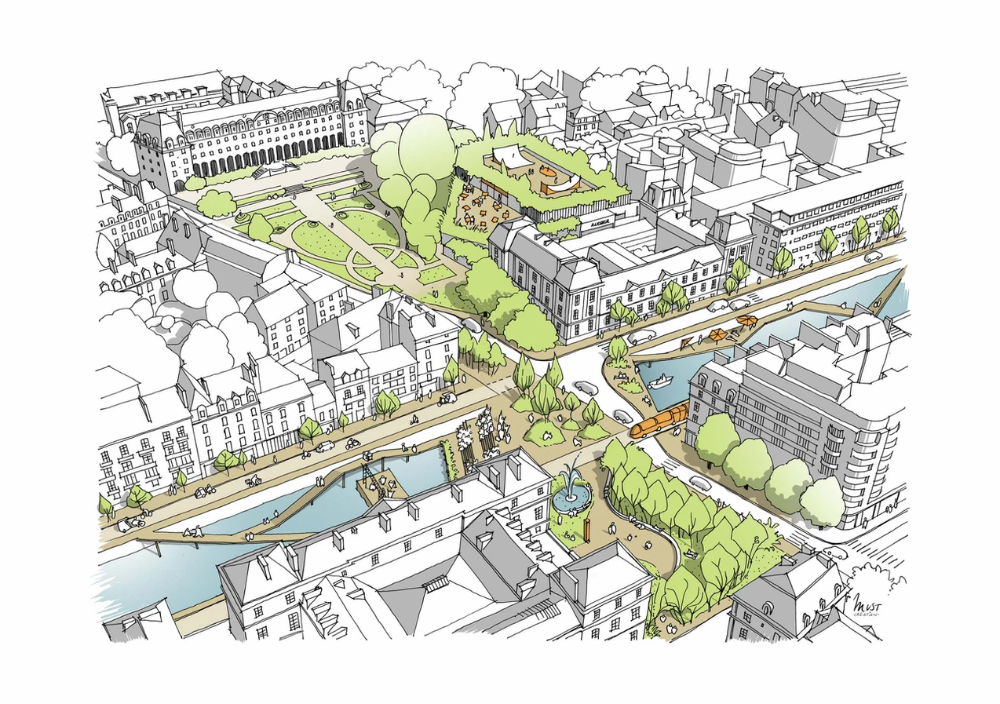
\includegraphics[scale=0.18]{centre-ville.png} \\
        \vspace{0.75cm}
      \end{center}
  \end{columns}
\end{frame}